\section{Рисование картинок \texttt{(physsummer-tikz)}}

В пакете собран инструментарий для рисования картинок при помощи \texttt{tikz}.

\dzcomment{
    Если при рисовании картинки вас тянет чего-то посчитать, например значение синуса какого-то угла, то
    скорее всего вы делаете что-то не так, и существует стандартное решение в \texttt{tikz}, которое
    сделает все за вас.
}


\subsection{Некоторые стандартные возможности \texttt{tikz}}

\subsubsection{Углы}

Ниже приведен пример отрисовки углов. Для задания угла необходимо иметь три точки, задаваемые при помощи
\texttt{coordinate} или \texttt{node}.

На третьем рисунке приведен пример того, что можно получить координату точки, где должна появиться
подпись угла, что может быть полезно, если необходимо залить область под подписью.

\begin{minipage}{0.28\linewidth}
    \begin{tikzpicture}[mstyle]
        \draw (2, 0) coordinate (a) -- (0, 0) coordinate (o)
            -- (60:2) coordinate (b);
        \pic[pic text = $\alpha$, draw = blue, angle eccentricity = 1.8, angle radius = 0.5cm]
            {angle = a--o--b};
        
        \draw (2, -6) coordinate (a1) -- ++(-2, 0) coordinate (o1)
            -- ++(60:2) coordinate (b1);
        \pic[pic text = $\beta$, style = double, draw = blue, angle eccentricity = 1.8, angle radius = 0.5cm]
            {angle = a1--o1--b1};
        
        \draw (2, -12) coordinate (a1) -- ++(-2, 0) coordinate (o1)
            -- ++(60:2) coordinate (b1);
        \pic (ver) [pic text = , draw = blue, angle eccentricity = 1.8, angle radius = 0.5cm]
            {angle = a1--o1--b1};
        \node[circle, inner sep = 2pt, fill = red!40] at (ver) {$\gamma$};
    \end{tikzpicture}
\end{minipage}
\begin{minipage}{0.72\linewidth}
    \begin{lstlisting}[gobble = 7]
        \begin{tikzpicture}
            \draw (2, 0) coordinate (a) -- (0, 0) coordinate (o)
                -- (60:2) coordinate (b);
            \pic[
                pic text = $\alpha$,
                draw = blue,
                angle eccentricity = 1.8,
                angle radius = 0.5cm]
                {angle = a--o--b};

            \draw (2, -6) coordinate (a1) -- ++(-2, 0) coordinate (o1)
                -- ++(60:1.2) coordinate (b1);
            \pic[
                pic text = $\beta$,
                style = double,
                draw = blue,
                angle eccentricity = 1.8,
                angle radius = 0.5cm]
                {angle = a1--o1--b1};

            \draw (2, -12) coordinate (a1)
                -- ++(-2, 0) coordinate (o1)
                -- ++(60:2) coordinate (b1);
            \pic (ver) [
                pic text = ,
                draw = blue,
                angle eccentricity = 1.8,
                angle radius = 0.5cm]
                {angle = a1--o1--b1};
            \node[circle, inner sep = 2pt, fill = red!40]
                at (ver) {$\gamma$};
        \end{tikzpicture}    
    \end{lstlisting}
\end{minipage}


\subsubsection{Пересечения  и касательные}

В \texttt{tikz} существуют встроенные средства для поиска пересечений кривых
\texttt{name intersections}. Для использования данной функции необходимо задать имена кривых при помощи
атрибута \texttt{name path}. После вызова функции точки пересечения получат имена \texttt{intersection-$i$}.

Во втором примере мы сразу проименовали точку пересечения, как \texttt{e}.

\begin{minipage}{0.28\linewidth}
    \begin{tikzpicture}[mstyle]
        \draw[thick, name path = ell] (0, 0) ellipse (2 and 1.5);
        \draw[name path = l1] (-2, -2) -- (2, 2);
        \path[name intersections = {of = ell and l1}];

        \node[above = 5pt] at (intersection-1) {$A$};
        \node[below = 5pt] at (intersection-2) {$B$};
        \draw[line width = 3pt, red] (intersection-1) -- (intersection-2);

        \draw[blue, thick, name path = line1] (-2, -3) -- (2, -5);
        \draw[blue, thick, name path = line2] (2, -3) -- (-2, -5);
        \path[name intersections = {of = line1 and line2, by = e}];
        \fill[red] (e) circle (0.07) node[above = 5pt, black] {$E$};
    \end{tikzpicture}
\end{minipage}
\begin{minipage}{0.72\linewidth}
    \begin{lstlisting}[gobble = 7]
        \begin{tikzpicture}
            \draw[thick, name path = ell] (0, 0) ellipse (2 and 1.5);
            \draw[name path = l1] (-2, -2) -- (2, 2);
            \path[name intersections = {of = ell and l1}];

            \node[above = 5pt] at (intersection-1) {$A$};
            \node[below = 5pt] at (intersection-2) {$B$};
            \draw[line width = 3pt, red] (intersection-1) --
                (intersection-2);

            \draw[blue, thick, name path = line1] (-2, -3) -- (2, -5);
            \draw[blue, thick, name path = line2] (2, -3) -- (-2, -5);
            \path[name intersections = {of = line1 and line2, by = e}];
            \fill[red] (e) circle (0.07)
                node[above = 5pt, black] {$E$};
        \end{tikzpicture}
    \end{lstlisting}
\end{minipage}


Похожим образом работает механизм построения касательных (работает только с ограниченным набором кривых),
с той лишь разницей, что вместо именования кривой, она должна быть задана при помощи \texttt{node}.

\begin{minipage}{0.28\linewidth}
    \begin{tikzpicture}[mstyle]
        \node[circle, draw, thick, minimum size = 2cm] (d1) at (0, 0) {};
        
        \coordinate (c) at (2, -2);
        \draw[very thick, red] (tangent cs:node = d1, point = {(c)}, solution = 1)
            node[above right, black] {$A$} -- (c) node[right, black] {$C$} --
            (tangent cs:node = d1, point = {(c)}, solution = 2) node[below, black] {$B$}; 
    \end{tikzpicture}
\end{minipage}
\begin{minipage}{0.72\linewidth}
    \begin{lstlisting}[gobble = 7]
        \begin{tikzpicture}
            \node[circle, draw, thick, minimum size = 2cm] (d1)
                at (0, 0) {};

            \coordinate (c) at (2, -2);
            \draw[very thick, red]
                (tangent cs:node = d1, point = {(c)}, solution = 1)
                node[above right, black] {$A$}
                -- (c) node[right, black] {$C$}
                -- (tangent cs:node = d1, point = {(c)}, solution = 2)
                node[below, black] {$B$};
        \end{tikzpicture}
    \end{lstlisting}
\end{minipage}


\subsubsection{Функции и циклы}

\texttt{tikz} предоставляет широкие возможности из классических языков программирования: условные
оператор, циклы, создание функций. В данном разделе мы продемонстрируем пример использования двух
последних конструкций.


\begin{minipage}{0.28\linewidth}
    \begin{tikzpicture}[mstyle]
        \tikzset{
            big-pic/.pic = {
                \foreach \a in {0, 1, ..., 100}{
                    \draw[red!\a!black, rotate around = {4 * \a:(0, 0)}] (-1, 0.5) -- (1, 0.5);
                }
                \fill (0, 0) circle (0.05);
                \draw[->, very thick] (0, 0) -- (400:0.5);
            }
        }
        
        \pic {big-pic};
        \pic[shift = {(0, -3)}, yscale = -1] {big-pic};
    \end{tikzpicture}
\end{minipage}
\begin{minipage}{0.72\linewidth}
    \begin{lstlisting}[gobble = 7]
        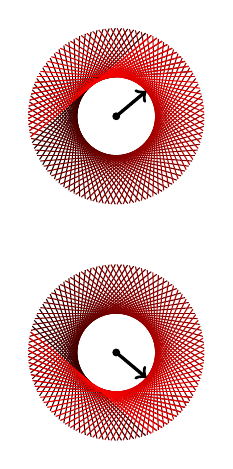
\begin{tikzpicture}
            \tikzset{
                big-pic/.pic = {
                    \foreach \a in {0, 1, ..., 100}{
                        \draw[
                            red!\a!black,
                            rotate around = {4 * \a:(0, 0)}]
                            (-1, 0.5) -- (1, 0.5);
                    }
                    \fill (0, 0) circle (0.05);
                    \draw[->, very thick] (0, 0) -- (400:0.5);
                }
            }

            \pic {big-pic};
            \pic[shift = {(0, -3)}, yscale = -1] {big-pic};
        \end{tikzpicture}
    \end{lstlisting}
\end{minipage}